\section{Hardware}

Here is the electrical schematic of our project:


\begin{figure}[H]
    \centering
    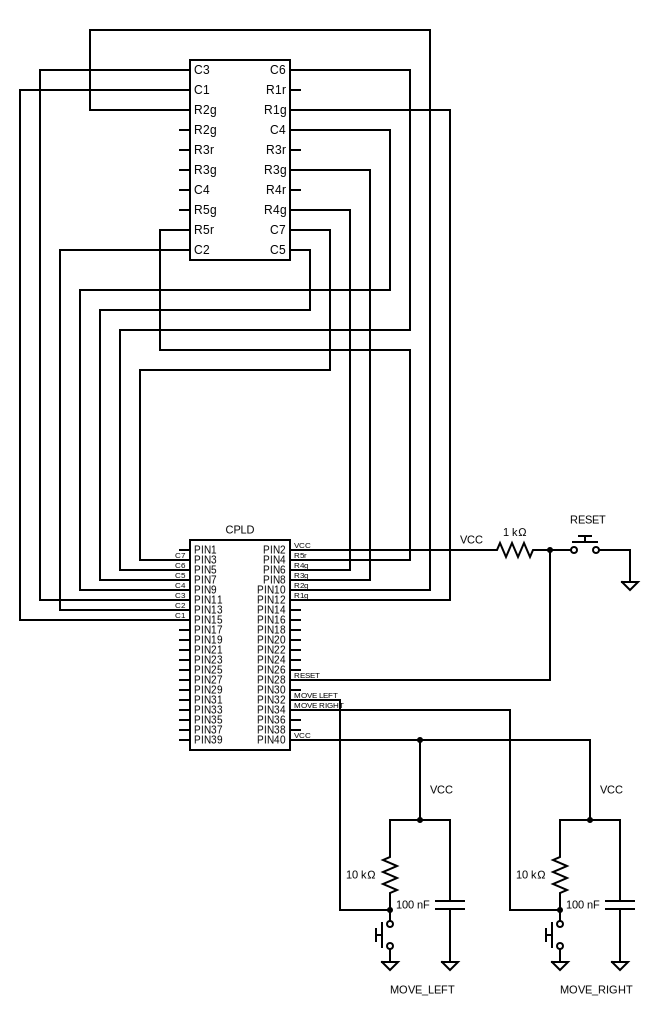
\includegraphics[scale = 0.4]{Ressources/png/circuit.png}
    \caption{Electrical schematics}
    \label{fig:my_label}
\end{figure}

The player needs three buttons to control the game. One to move the paddle to the left, another one to move it to the right and the last one to start/reset the game. Here is the explanation of how they work :  \\
\begin{itemize}

    \item[$\bullet$] \textbf{Move buttons:} The buttons have to be pushed to move the paddle. It means that it detects when \texttt{MOVE\_LEFT} = '0' or if \texttt{MOVE\_RIGHT} = '0'. As represented in the schematic, when a button is pushed, the input voltage is the ground so it is why we have '0'. To make sure that we do not have any voltage bounces, each button is in series with a 10 $k\Omega$ resistance and in parallel with a 100 nF capacitor. \\

    \item[$\bullet$] \textbf{Reset button:} This button has to be pushed to start playing, to play again if you have lost or to reset the game while you are playing. It is also in series with a 10 $k\Omega$ resistance and in parallel with a 100 nF capacitor. It works like the two other buttons : if you push it, the voltage goes to the ground and the input signal \texttt{START} = '0'. When reset button is pressed, the game starts again with 3 lives. \\
\end{itemize}

For the LED matrix, we used a bi-color 5 x 7 LED matrix \href{https://www.kingbrightusa.com/images/catalog/SPEC/TBC20-11EGWA.pdf}{(TBC20-11EGWA)}. We used 12 of the 20 pins available. For the 4 first rows, we used the green LEDs and for the last row (the bottom one) we used the red LEDs.

\begin{center}
\begin{tabular}{|c|c|c|}
\hline
\multicolumn{3}{|c|}{LED to chip pin assignment}\\
\hline
Name & pin on the CPLD & location on the chip \\
\hline
Row 1 green & pin 12 & pin 1 \\
\hline
Row 2 green & pin 10 &  pin 2\\
\hline
Row 3 green  & pin 8 &  pin 3\\
\hline
Row 4 green & pin 6 & pin 4\\
\hline
Row 5 red & pin 4 & pin 5\\
\hline
Column 1 & pin 15 & pin 56\\
\hline
Column 2 & pin 13 & pin 58\\
\hline
Column 3 & pin 11 & pin 59\\
\hline
Column 4 & pin 9 & pin 60 \\
\hline
Column 5 & pin 7 & pin 61\\
\hline
Column 6 & pin 5 & pin 62\\
\hline
Column 7 & pin 3 & pin 63\\

\hline
\end{tabular}
\label{table_1}
\end{center}